\chapter{Background}

The classical approach to extract useful information from an image has been to find mathematical definitions for features that describe the information. The features could, for example, be lines, circles, or edges. 
Circles can be used to find coins, where the diameter denotes the value. Lines can be used to find how many fenceposts are in a fence. Traditional mathematical models include the Hough Transform~\cite{houghTransform} for detecting lines or circles, the Sobel operator to detect gradients, and in return, edges, or the Gray Level Co-occurrence Matrix for detecting texture features. 
In common for all these methods is that they are well defined and find precisely \emph{one} type of feature that was previously specified. 
At a higher level, hand-crafted feature descriptors have been made. They look for a specific set of features in an image to identify unique locations. Some well-known examples are the SIFT~\cite{sift1999Lowe}, SURF~\cite{surf2006Bay} and ORB~\cite{orb2011Rublee} feature descriptors. They have been used successfully in applications such as combining images into panoramas or combining different views to a 3D model, also known as Structure from motion~\cite{sfm1979ullman}.

Hand-crafted features have also been used in machine learning scenarios. As an example, Haar-like features were demonstrated to efficiently find faces in \cite{haarcascade}. Here, the machine learning model decided which of a given set of features to use to classify whether the frame contained a face or not. In using both the Sobel operator and using Haar-like features, a filter is passed over the image. In the case of the Sobel operator, this is an actual convolution of the image with the filter, whereas Haar-features are extracted using a sliding window. This is the intuition that is used in Convolutional Neural Networks, discussed next.

\section{Convolutional Neural Networks}\label{sec:background_cnn}
First introduced by Fukushima~\cite{Fukushima1980} \gls{cnn}s encode spatial information without being affected by shifts in the position of that information. In other words, they look at collections of \emph{spacially connected pixels}. \gls{cnn}s use filters, or kernels, to extract features that help them to ``understand'' an image. The deeper the network is, the more complex features emerge. In addition, the \emph{receptive field}, the patch of the original image that affects the feature, becomes larger. 

Instead of using hand-crafted features, deep \gls{cnn}s define the features they use when they are trained. This is one of the reasons why \gls{cnn}s needs fairly large training sets, as well as taking a long time to train. Therefore, a popular approach is to reuse the first few primitive layers (the first layers encountered in a forward-pass) from other models. This is known as \emph{Transfer Learning}. It can be accomplished by first training a neural network for a specific task, for example, recognizing a handful of different types of objects in an image. Then, the primitive layers with their parameters are ``chopped off'' the network. Since these layers only have learned primitive features, these learned features can be input and fine-tuned to specialize a different network, which in turn needs less training time since it has already learned the simple features. Another advantage of this is that the two networks can be trained on vastly different datasets. If one application area has an abundance of training data, the first network could be trained on this. As long as the general input is the same, namely the number of channels and the values presented, the first few layers can be easily fine-tuned to a new application area.

When designing a \gls{cnn}, it is often helpful to have in mind exactly what one can imagine should be detected in each layer. In 2D images, the first few layers of a deep \gls{cnn} have been shown to often mimic the behavior of the simple handmade feature extractors such as the ones discussed above. However, such features can be quite different in 3D. Instead of edge-detectors, one can imagine plane detectors or other detectors unique to 3D objects. Additionally, 3D depth images only have a single channel, whereas most 2D \gls{cnn}s have been trained on 3-channel RGB images. \cite{song2018depth} argues that it is, therefore, better to train such networks from scratch.

\begin{figure}[h]
  \centering
  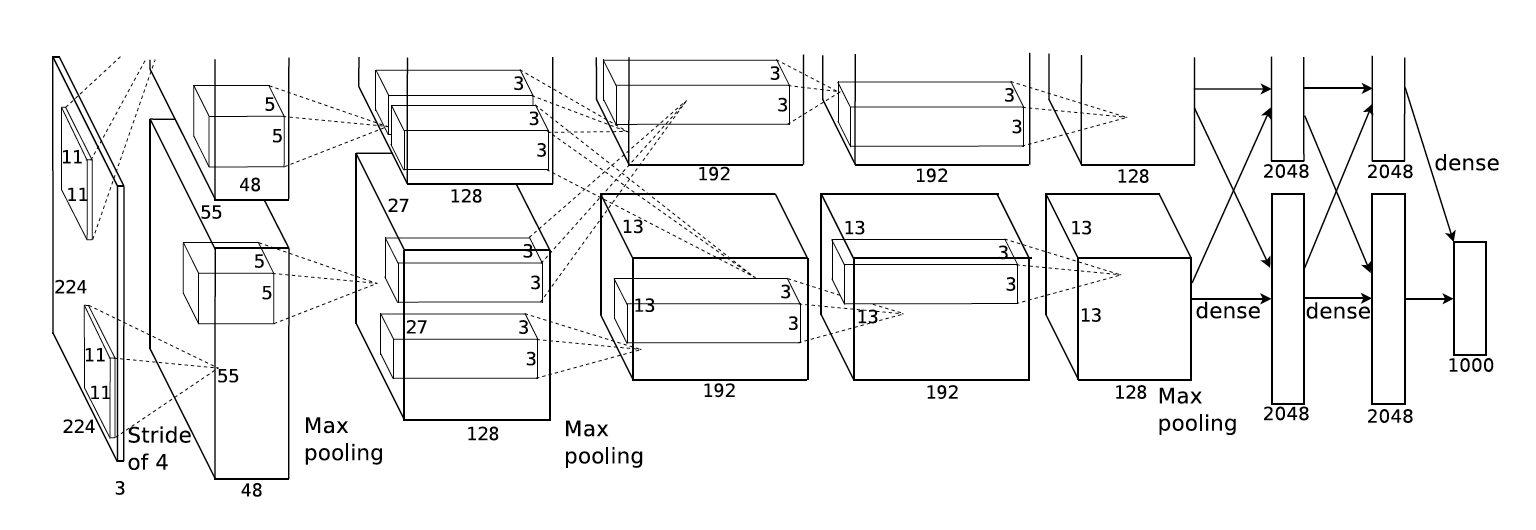
\includegraphics[width=\textwidth]{img/alexnet}
  \caption[AlexNet]{Illustration of a Convolutional Neural Network. The figure is borrowed from AlexNet~\cite{alexnet2012}}
  \label{fig:alexnet}
\end{figure}

\section{Depth Images}
In contrast to color, or RGB images, depth images contain information about the distances. Each pixel contains a measure of the distance from the camera x,y plane to the real world point projected through that pixel. 

%% TODO> about loss of accuracy at distance

%% TODO> about reprojection from world to image-coordinates



\section{Pose Estimation}
Human Pose Estimation is an area well-researched area because of its many applications. Much of the research focuses on finding pose in RGB images, where hand-crafted features such as parallel edges \cite{ramanan2003,mori2002}, silhouette features \cite{grauman2003}, or pictorial structures \cite{fischler1973,felzenszwalb2005}, have been used to suggest candidates for limbs, joints, and so on. From such evidence, constrained kinematic models, tree graphs, or decision trees \cite{shotton2013}, are used to construct the poses with varying degrees of success. With such top-down approaches, will the runtime of the algorithm increase when multiple people are present in the image.

With the increasing popularity of \gls{cnn}s in recent years, many techniques utilizing them have also been developed for human pose estimation \cite{tompson2014joint}. A particularly popular approach is to use a deep \gls{cnn} to produce heat-maps that suggest candidate locations for various body parts \cite{wei2016cpm,wang2016}.

Much research has been done in estimating human pose in two dimensions, as quite large datasets have been made such, as the MPII, or the Human 3.6M datasets \cite{andriluka14cvpr,h36m_pami}.

The other approach is to use object recognition to find key features for the whole image. Then the recognized landmarks are combined to build up the people instances.

In \cite{cao2017realtime}, the second approach is used. Two \gls{cnn}s, one for landmark localization and the other for recombination, are trained to estimate human pose. One of the networks produces a \emph{confidence map} for each joint. Each pixel in the confidence map contains the probability, or confidence, that the pixel is part of a person's joint. The other creates \gls{paf}s, which is a map of vectors pointing in the direction of one of \emph{M} limbs. \footnote{This work will stick to the convention of using the term \emph{limb} to describe any \emph{connection between any pair of body landmarks}. The body landmarks will be termed \emph{joints}.} These maps are assembled by bipartite matching to create the 2D skeletons observed in the scene.

\begin{figure}[h]
  \captionsetup[sub]{font=scriptsize,belowskip=2pt,aboveskip=3pt}
  \begin{subfigure}[t]{0.24\textwidth}
    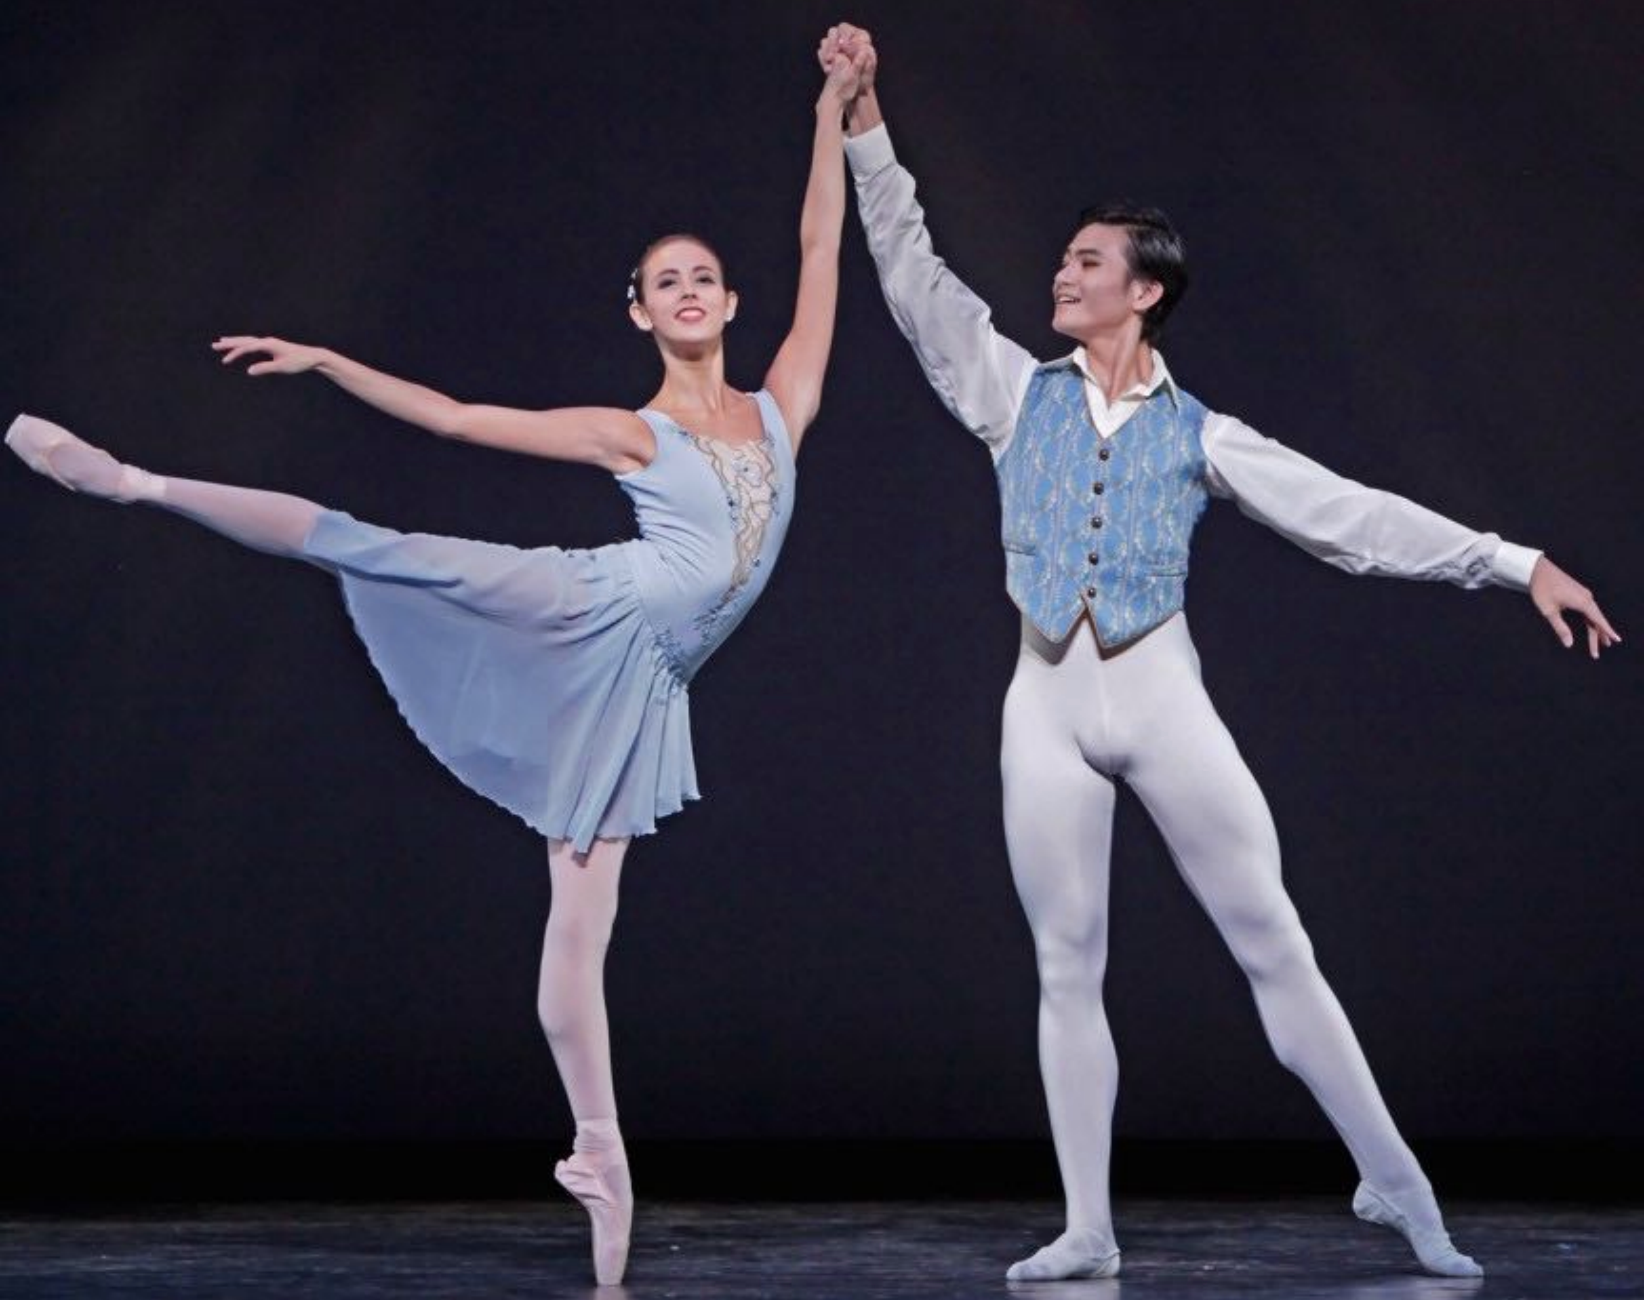
\includegraphics[width=1\linewidth]{img/openpose_pipeline_a}
    \caption{Input Image}
    \label{fig:oppA}
  \end{subfigure}%
  ~
  \begin{subfigure}[b]{0.24\textwidth}
    \begin{subfigure}{1\textwidth}
      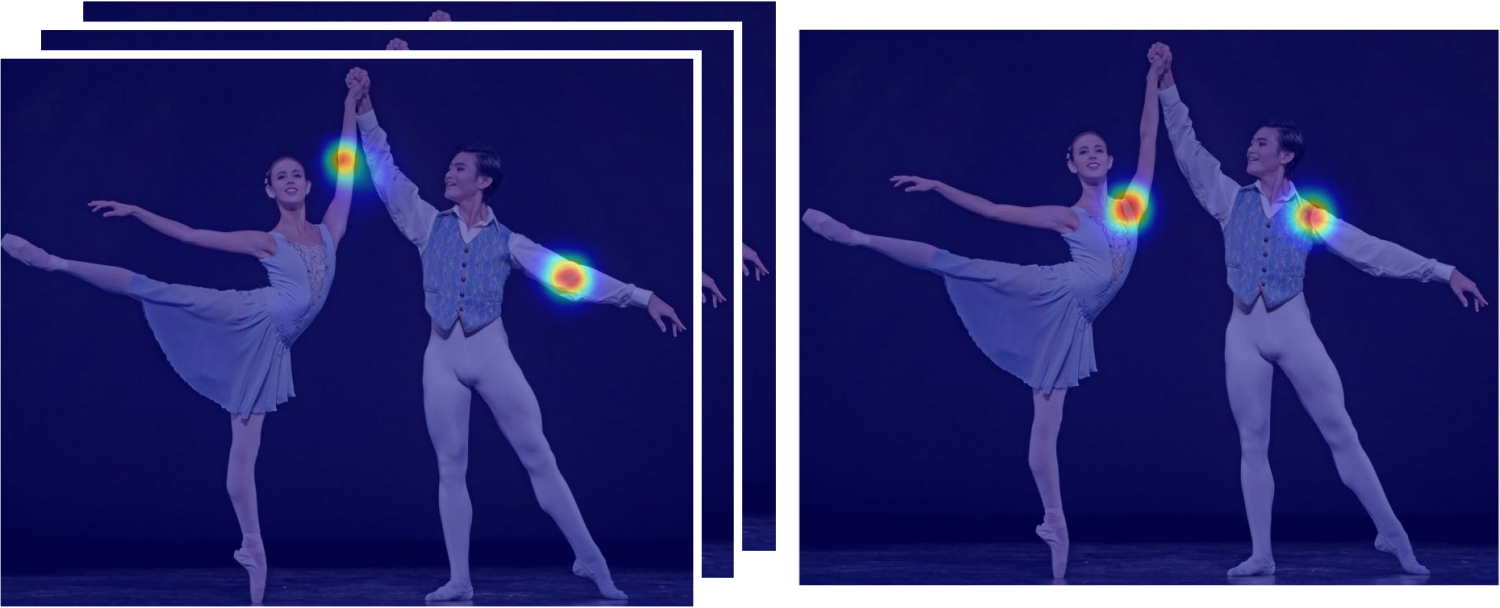
\includegraphics[width=1\linewidth]{img/openpose_pipeline_b}
      \caption{Part Confidence Maps}
      \label{fig:oppB}
    \end{subfigure}
    
    \begin{subfigure}{1\textwidth}
      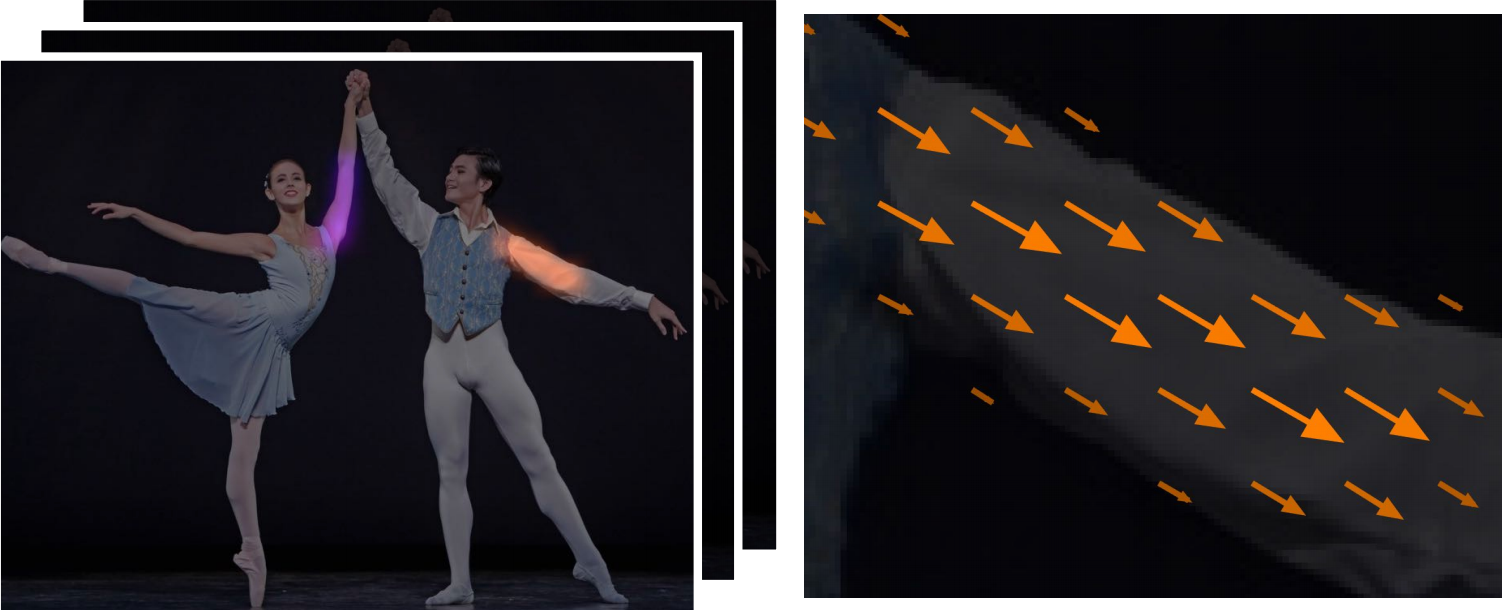
\includegraphics[width=1\linewidth]{img/openpose_pipeline_c}
      \caption{Part Affinity Fields}
      \label{fig:oppC}
    \end{subfigure}
  \end{subfigure}%
  ~
  \begin{subfigure}[t]{0.24\textwidth}
    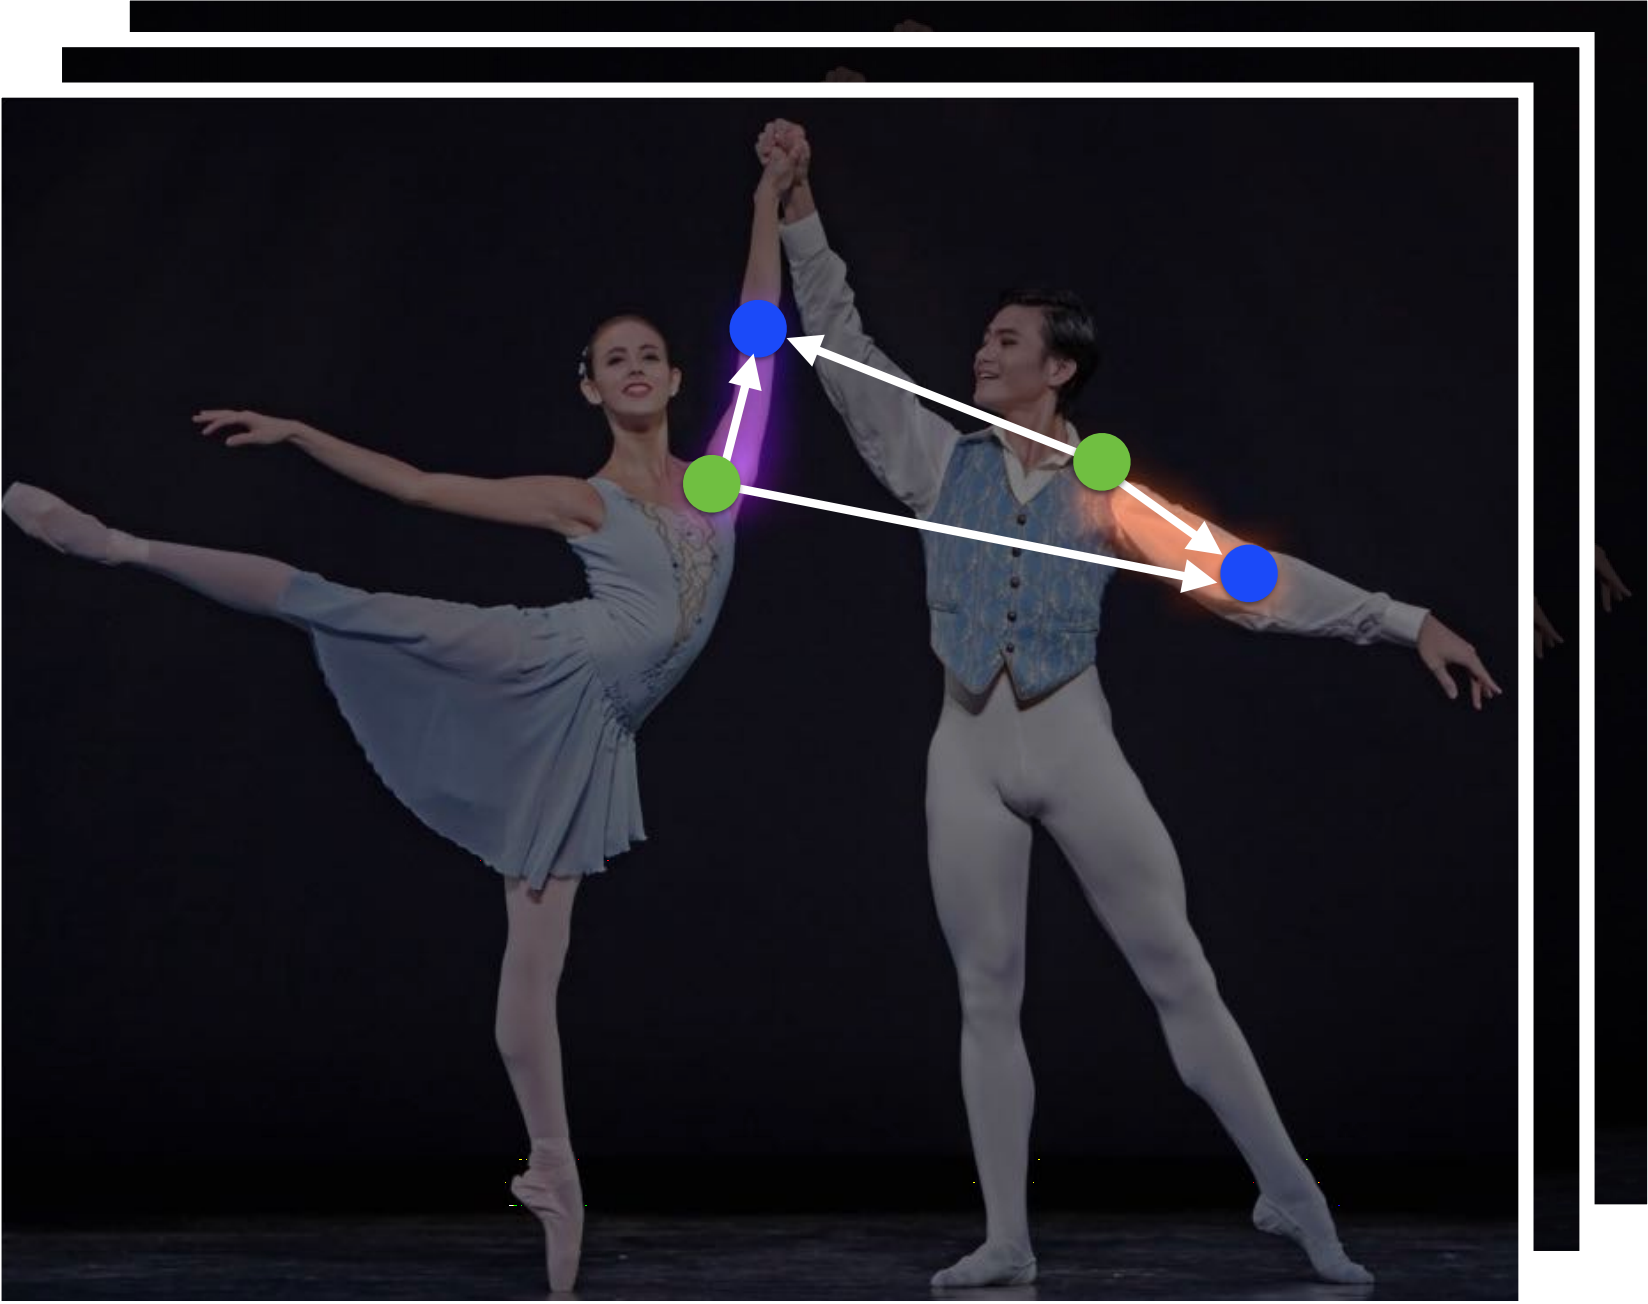
\includegraphics[width=1\linewidth]{img/openpose_pipeline_d}
    \caption{Bipartite Matching}
    \label{fig:oppD}
  \end{subfigure}%
  ~
  \begin{subfigure}[t]{0.24\textwidth}
    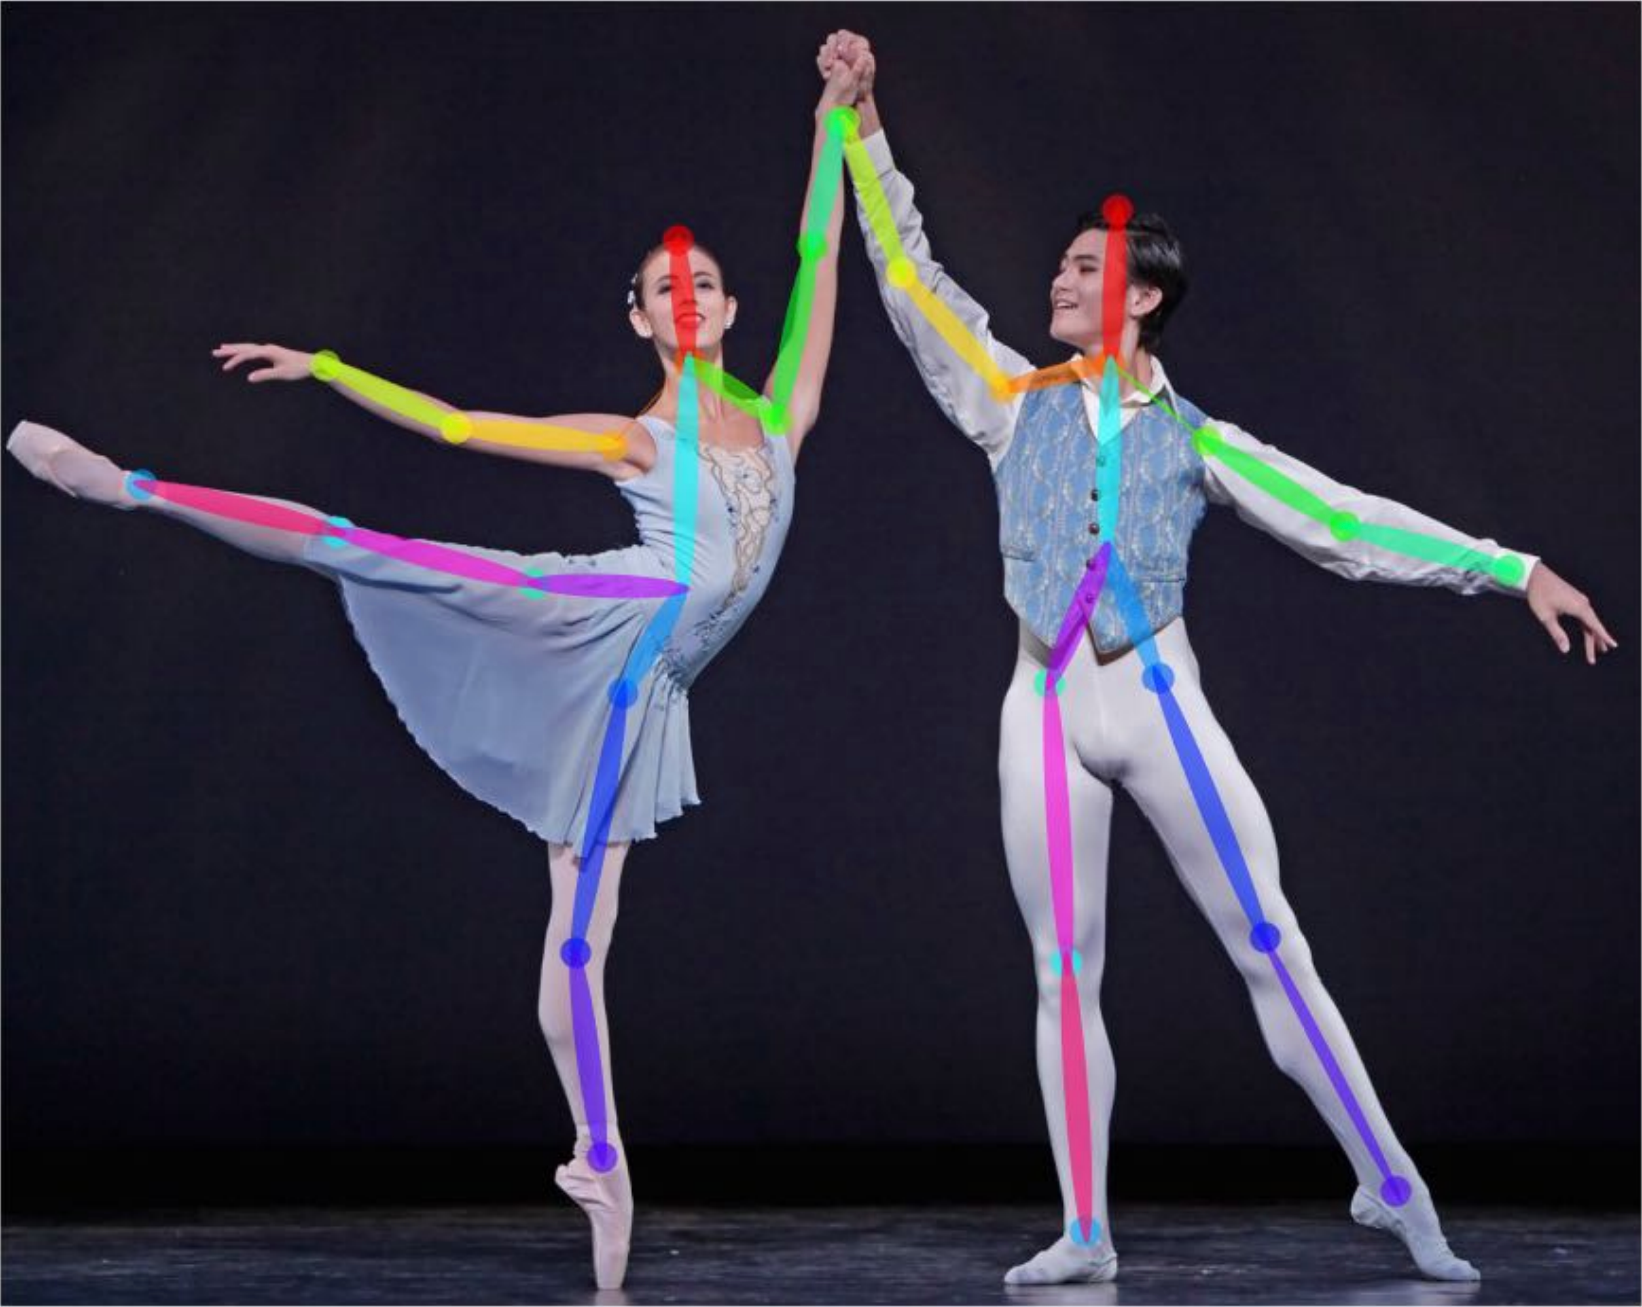
\includegraphics[width=1\linewidth]{img/openpose_pipeline_e}
    \caption{Parsing Results}
    \label{fig:oppE}
  \end{subfigure}
  \caption[OpenPose pipeline]{The pipeline used in OpenPose~\cite{cao2017realtime, cao2019openpose}. The input image \ref{fig:oppA} is fed into the two networks, which produce joint detections in confidence maps \ref{fig:oppB} and PAFs  \ref{fig:oppC}. Bipartite matching is performed in \ref{fig:oppD}, to determine which detected joints should be connected by a limb. \ref{fig:oppE} shows the finished results.}
  \label{fig:openpose_pipeline}
\end{figure}

Using the method described in \cite{cao2017realtime}, no information is given for joints that are not accurately detected. If, for example, an extremity is occluded together with half of the connecting limb, the extremity will not be part of the output skeleton, even if the joint could be extrapolated from the parts of the limb that is visible.
This is also true for undetected joints in the middle of a joint chain. The joint could be extrapolated using the surrounding joints. The problem with joint-extrapolation happens because of the bipartite matching, which does not work if any joint is missing.



